%%% Local Variables: 
%%% coding: utf-8
%%% mode: latex
%%% TeX-engine: xetex
%%% End: 

\documentclass[hide notes,intlimits]{beamer}
\mode<presentation>
{
  \usetheme[footline]{PISMshade}
  \setbeamercovered{transparent}
}

% load packages
\usepackage{media9}
\usepackage[english]{babel}
\usepackage[multidot]{grffile}

\usepackage{tikz}
\usetikzlibrary{shapes,arrows}
\usetikzlibrary{shadows}

\definecolor{dark red}{HTML}{E41A1C}
\definecolor{dark green}{HTML}{4DAF4A}
\definecolor{dark violet}{HTML}{984EA3}
\definecolor{dark blue}{HTML}{084594}
\definecolor{dark orange}{HTML}{FF7F00}
\definecolor{light blue}{HTML}{377EB8}
\definecolor{light red}{HTML}{FB9A99}
\definecolor{light violet}{HTML}{CAB2D6}

\setbeamercolor{boxed}{fg=black,bg=light blue!25}
\graphicspath{{figures/}{../2022_04_igs/figures/}{../figures/}{../figures_2018_08/}{../2021_09_cph/figures/}{../2021_11_geo/figures/}}


\newcommand{\jl}{[\![}
\newcommand{\jr}{]\!\hskip 0.003cm ]}
\newcommand{\bpsi}{\boldsymbol{\psi}}
\newcommand{\bPsi}{\boldsymbol{\Psi}}
\newcommand{\bphi}{\boldsymbol{\phi}}
\newcommand{\bPhi}{\boldsymbol{\Phi}}
\newcommand{\bn}{\mathbf{n}}
\newcommand{\bq}{\mathbf{q}}
\newcommand{\bv}{\mathbf{v}}
\newcommand{\D}{\,\mathrm{d}}
\newcommand{\Tsnow}{T_{\text{snow}}}
\newcommand{\Hatm}{H_{\text l}^{\text{atm}}}

\newcommand{\mathtext}[1]{\mathsf{#1}}

% title page
\title[Ice sheet modeling] % (optional, use only with long paper titles)
{A reanalysis of the Greenland Ice Sheet}
\author[Aschwanden] % (optional, use only with lots of authors)
{\textbf{Andy Aschwanden}\\ with \\Doug Brinkerhoff, Mark Fahnestock}
\institute{Geophysical Institute, University of Alaska Fairbanks}

% - Give the names in the same order as the appear in the paper.
% - Use the \inst{?} command only if the authors have different
%   affiliation.

% - Use the \inst command only if there are several affiliations.
% - Keep it simple, no one is interested in your street address.
\titlegraphic{\vskip-.5cm
\includegraphics[height=1.5cm]{pism_logo_v2_transp}}

\date{}


\subject{Credible sea-level projections}

\begin{document}


\setbeamertemplate{background canvas}
  {
}

 
% insert titlepage
\begin{frame}
  \titlepage
\end{frame}

\setbeamertemplate{background canvas}
  {
}


\begin{frame}{Motivation}
  \begin{figure}
    \includegraphics<1>[width=.9\textwidth]{ar6_wg1_fig_9_17_draft_with_zoom}
    \caption{IPCC AR6 Draft, Fig. 9.17}
  \end{figure}
\end{frame}


\begin{frame}
  \frametitle{Summary}
  Our goal is
  \begin{itemize}
    \item to adapt data assimilation strategies from numerical weather predictions to numerical ice sheet predictions
    \item to create a reanalysis of the Greenland Ice Sheet
  \end{itemize}
\end{frame}

\part{How did we get here?}
\frame{\partpage}


\begin{frame}
  \frametitle{The 1990s}
      \begin{figure}
        \includegraphics<1>[width=\textwidth]{greve-1995}
      \end{figure}
\end{frame}

\begin{frame}
  \frametitle{The 1990s}
      \vspace{-2em}
  \begin{columns}[c]
    \begin{column}{.5\linewidth}
    \begin{figure}
      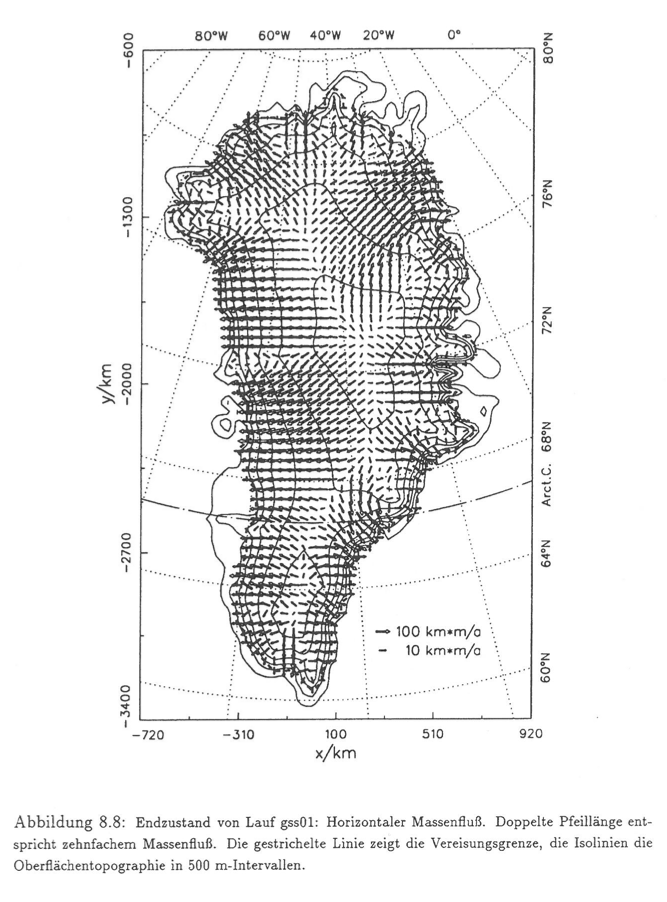
\includegraphics[height=0.75\textheight]{greve_1995_flow}\\
      \tiny{Greve, 1995}
    \end{figure}
    \end{column}
    \begin{column}{.4\linewidth}
      \begin{figure}
      \includegraphics[height=.7\textheight]{greenland-obs-rignot}\\
      \tiny{Rignot \& Mouginot, 2012}
      \end{figure}
    \end{column}
  \end{columns}
\end{frame}


\begin{frame}
  \frametitle{IPCC AR3, 2001}
  \begin{columns}[c]
    \begin{column}{.4\linewidth}
      \begin{figure}
        \includegraphics[height=5cm]{ar3-wg1}
      \end{figure}
    \end{column}
    \begin{column}{.5\linewidth}
      \begin{itemize}
        \item 1 ice sheet model (?)
        \item ``The Antarctic ice sheet is likely to gain mass, while the Greenland ice sheet is likely to lose mass''
        \item ``However, loss of grounded ice leading to substantial sea level rise from WAIS is now widely agreed to be very unlikely during the 21st century''
      \end{itemize}
    \end{column}
\end{columns}
\end{frame}


\begin{frame}
  \frametitle{IPCC AR4, 2007}
  \begin{columns}[c]
    \begin{column}{.4\linewidth}
      \begin{figure}
        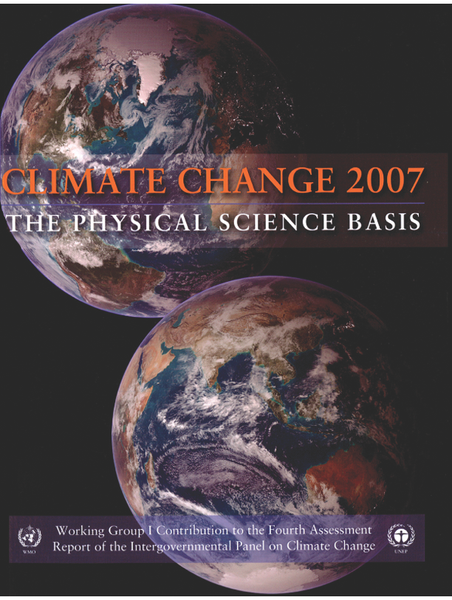
\includegraphics[height=5cm]{ar4-wg1}
      \end{figure}
    \end{column}
    \begin{column}{.5\linewidth}
      \begin{figure}
        
\includegraphics[height=3.5cm]{no-ice-sheet-models}
      \end{figure}
      \begin{itemize}
      \item No results from ice sheet models included due to the models' inability to track recent changes
      \end{itemize}
    \end{column}
\end{columns}
\end{frame}


\begin{frame}{Observed vs simulated flow speeds (2007 model)}
  \begin{columns}[c]
    \begin{column}{.6\linewidth}
    \begin{figure}
      \includegraphics[height=5.75cm]{gris-obs-exp-old}
      \\ \tiny{adapted from Aschwanden, Fahnestock, Truffer (2016) \textit{Nature Comms.}}
    \end{figure}
    \end{column}
    \begin{column}{.4\linewidth}
      \begin{figure}
        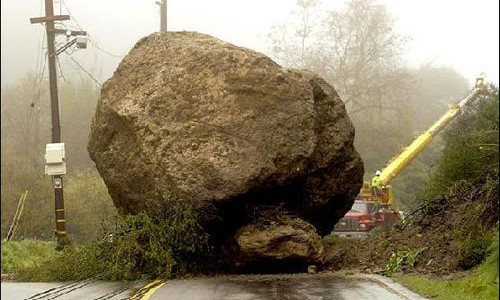
\includegraphics[width=.75\textwidth]{roadblocks}
      \end{figure}
      \begin{itemize}
      \item can't reproduce the velocity field
      \item this led to a model development frenzy
      \end{itemize}
    \end{column}
  \end{columns}
  \note[item]{}
\end{frame}

\begin{frame}{The post AR4 world: Stokes models}
  \begin{columns}[c]
    \begin{column}{.6\linewidth}
    \begin{figure}
      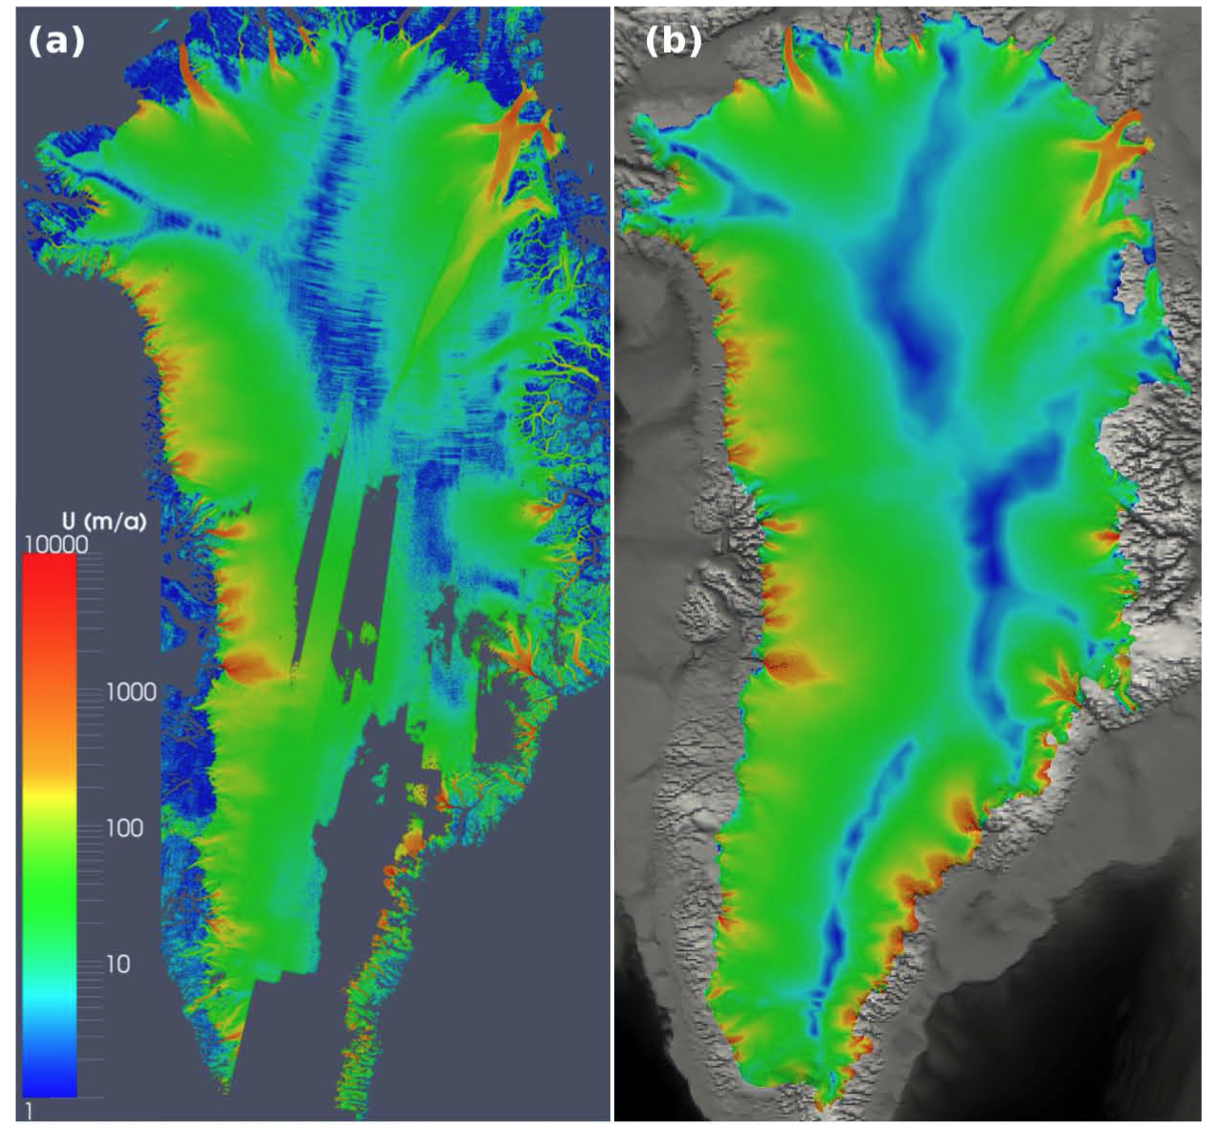
\includegraphics[height=7cm]{gillet-chaulet_2012_fig_1}
      \\ \tiny{Gillet-Chaulet et al. (2012)}
    \end{figure}
    \end{column}
    \begin{column}{.4\linewidth}
      \begin{figure}
        
\includegraphics[width=.75\textwidth]{elmer}
        
\includegraphics[width=.75\textwidth]{issm}
      \end{figure}
    \end{column}
  \end{columns}

\end{frame}

\begin{frame}{The post AR4 world: Data Assimilation}
    \begin{figure}
      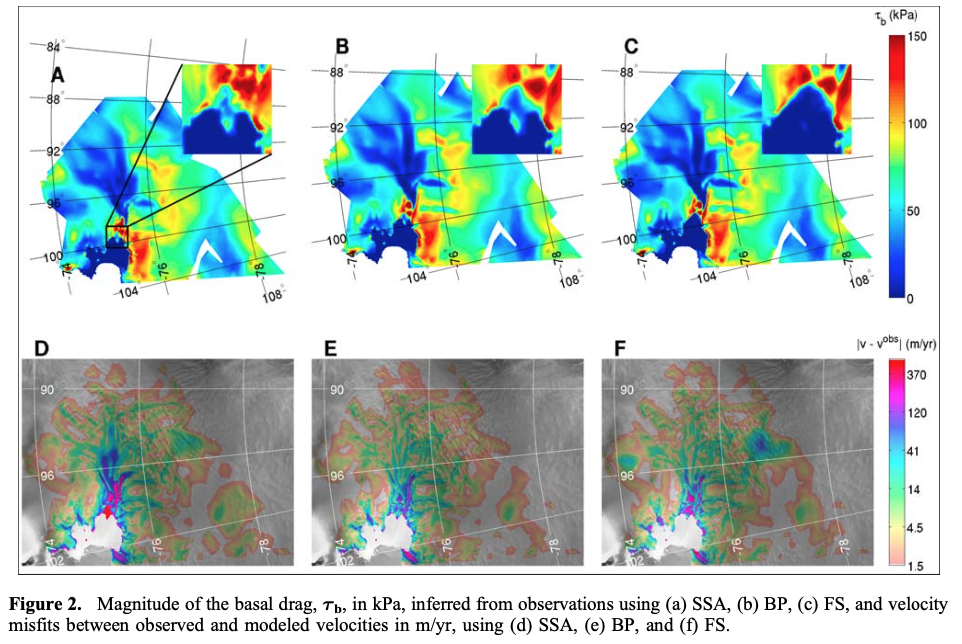
\includegraphics[height=7cm]{morlighem_2010_fig_2}
      \\ \tiny{Morlighem et al. (2010)}
    \end{figure}
\end{frame}

\begin{frame}{The post AR4 world: Data Assimilation}
    \begin{figure}
      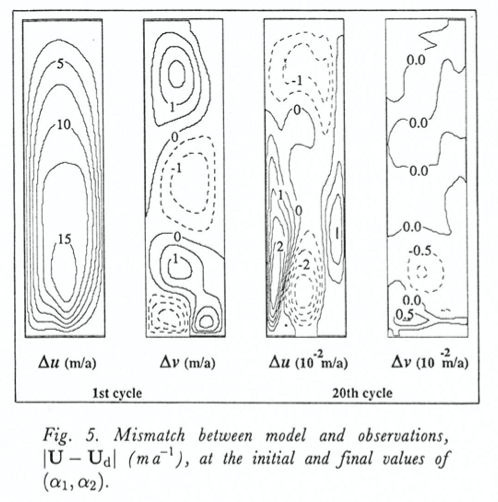
\includegraphics[height=7cm]{macayeal_1993_fig_5}
      \\ \tiny{MayAyeal (1993)}
    \end{figure}
\end{frame}

\begin{frame}{The post AR4 world: Sensitivity Analysis}
    \begin{figure}
      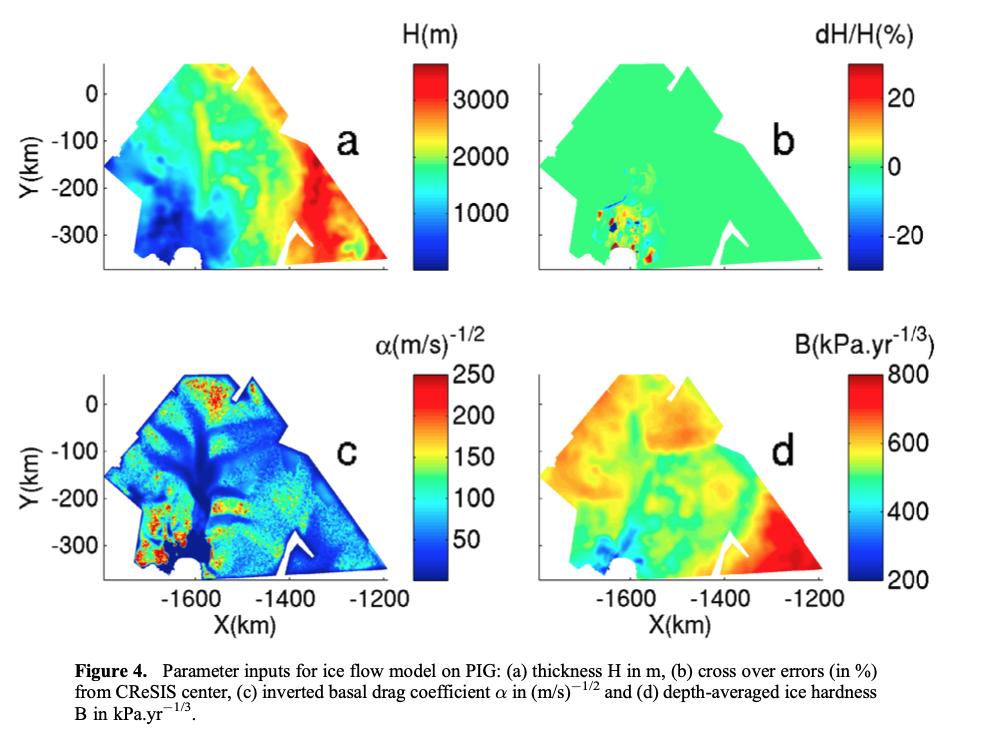
\includegraphics[height=7cm]{larour_2012_fig_4}
      \\ \tiny{Larour et al. (2012)}
    \end{figure}
\end{frame}


\begin{frame}{The post AR4 world: Observations}
  \begin{figure}
    \includegraphics<1>[height=3cm]{grace-satellites} \vspace{0.5em}
    \includegraphics<1>[height=3cm]{sentinel-satellites}
    \\[.5em]
    \includegraphics<1>[height=3cm]{oib}
  \end{figure}
  Data rich(er)
\end{frame}


\begin{frame}
  \frametitle{IPCC AR5, 2013}
  \begin{columns}[c]
    \begin{column}{.4\linewidth}
      \begin{figure}
        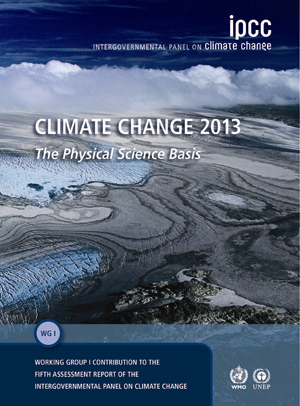
\includegraphics[height=5cm]{ar5-wg1}
      \end{figure}
    \end{column}
    \begin{column}{.6\linewidth}
      \begin{figure}
        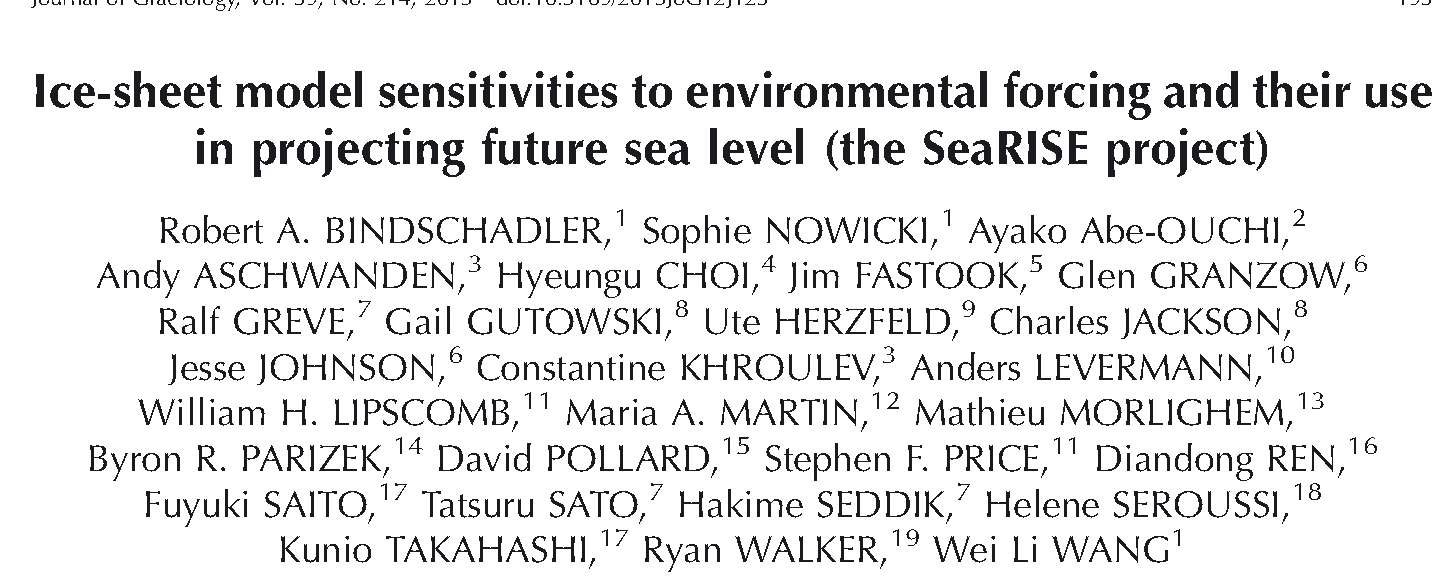
\includegraphics[width=4.75cm]{searise}
      \end{figure}
      \begin{figure}
        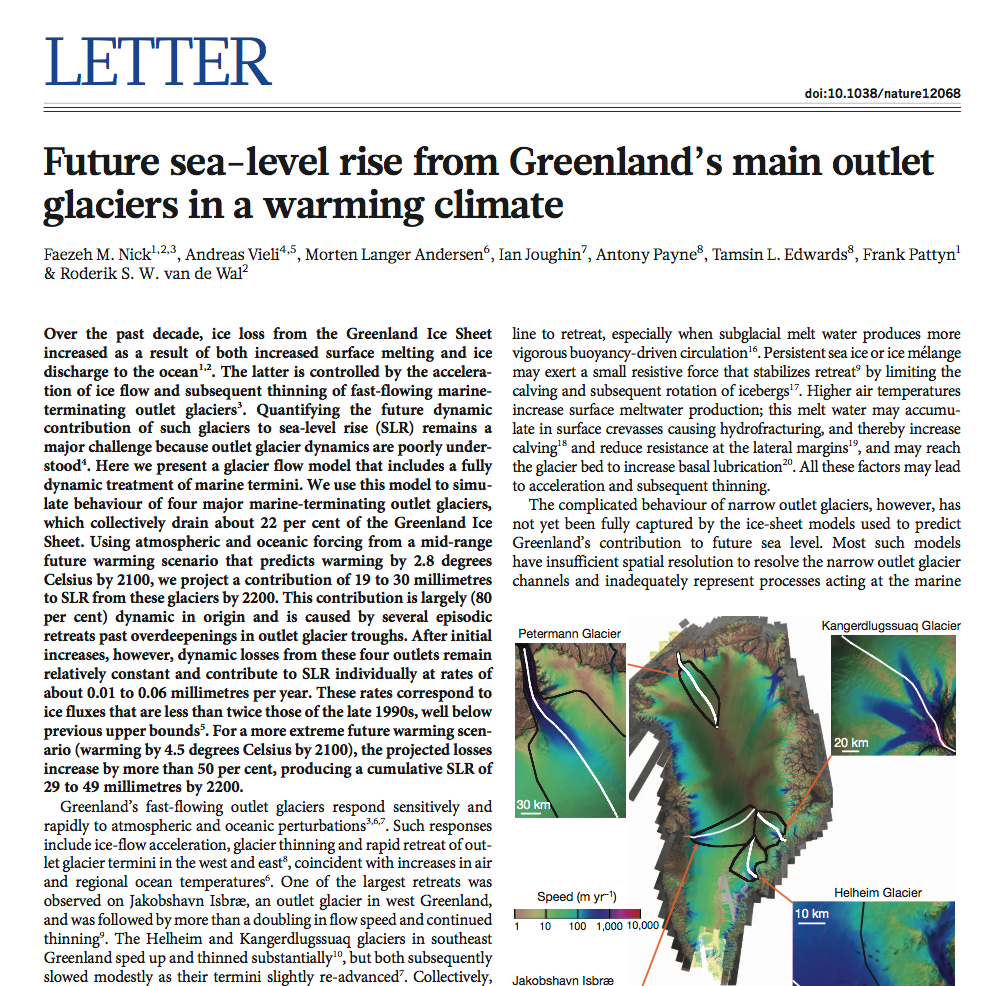
\includegraphics[width=4.75cm]{nick2013}
      \end{figure}
    \end{column}
  \end{columns}
\end{frame}

\begin{frame}{Observed vs simulated flow speeds (2013 model)}
  \alert{Have the models gotten any better? Not really.}
  \begin{columns}[c]
    \begin{column}{.6\linewidth}
    \begin{figure}
      \includegraphics[height=5.75cm]{gris-obs-exp-old}
      \\ \tiny{adapted from Aschwanden, Fahnestock, Truffer (2016) \textit{Nature Comms.}}
    \end{figure}
    \end{column}
    \begin{column}{.4\linewidth}
      \begin{figure}
        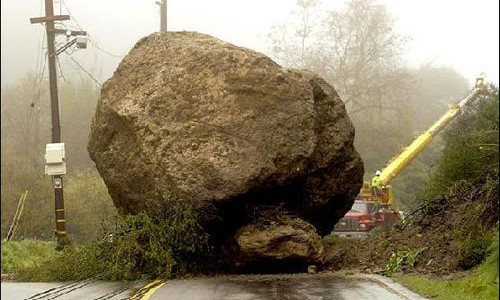
\includegraphics[width=.75\textwidth]{roadblocks}
      \end{figure}
      \begin{itemize}
      \item still can't reproduce the velocity field
      \end{itemize}
    \end{column}
  \end{columns}
  \note[item]{}
\end{frame}

\begin{frame}{Post AR5 models}
  \alert{Have the models gotten any better? Yes. Finally.}
  \begin{columns}[c]
    \begin{column}{.6\linewidth}
    \begin{figure}
      \includegraphics[height=5.75cm]{gris-obs-exp-new}
      \\ \tiny{adapted from Aschwanden, Fahnestock, Truffer (2016) \textit{Nature Comms.}}
    \end{figure}
    \end{column}
    \begin{column}{.4\linewidth}
      \begin{figure}
        % 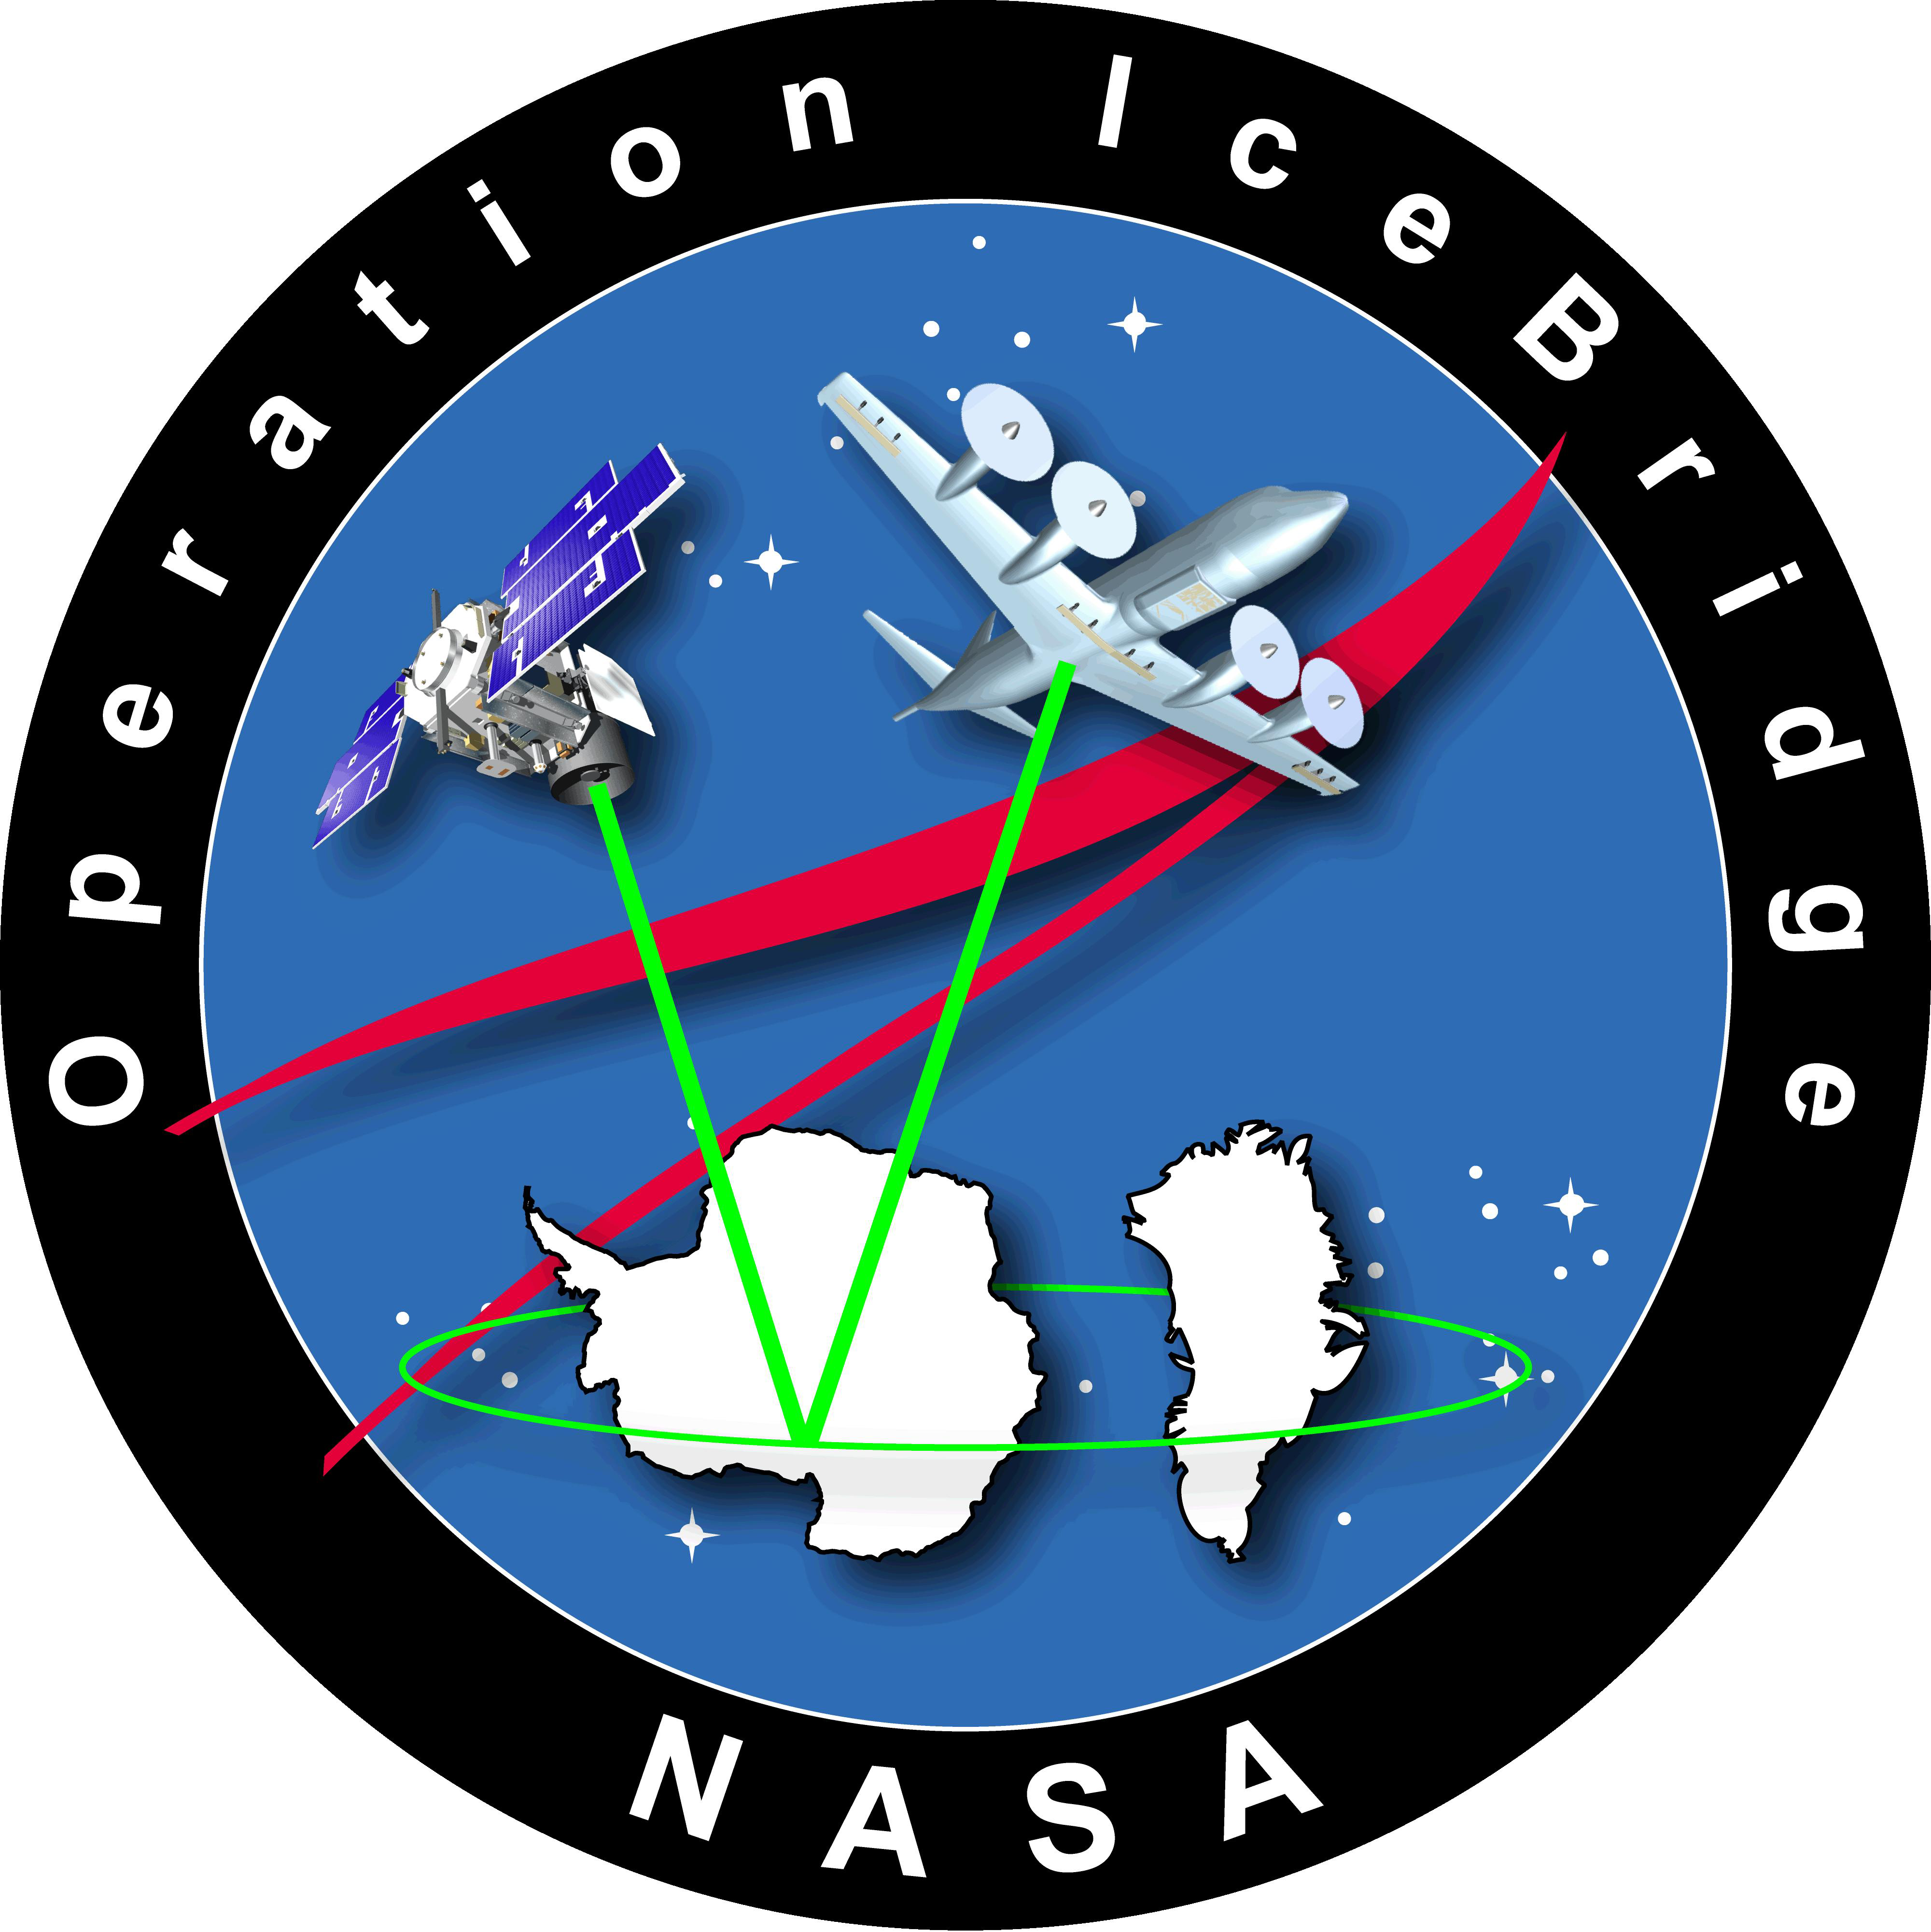
\includegraphics[height=1cm]{oib} \\
        \includegraphics[height=5.75cm]{greenland-bed-mcb}
      \\ \tiny{adapted from Morlighem et al. (2014) \textit{Nature Geosci.}}
      \end{figure}
    \end{column}
  \end{columns}
  \alert{Accurate ice thickness does the trick}
  
  \note[item]{first time capturing the flow field for the right reason}
  \note[item]{this is quite a break through in ice sheet modeling}
  \note[item]{though not a surprising one}
  \note[item]{it just confirms what students learn in glaciology 100:}
  \note[item]{ice flows downhill}
\end{frame}


\begin{frame}
  \frametitle{IPCC AR6, 2021}
  \begin{columns}[c]
    \begin{column}{.4\linewidth}
      \begin{figure}
        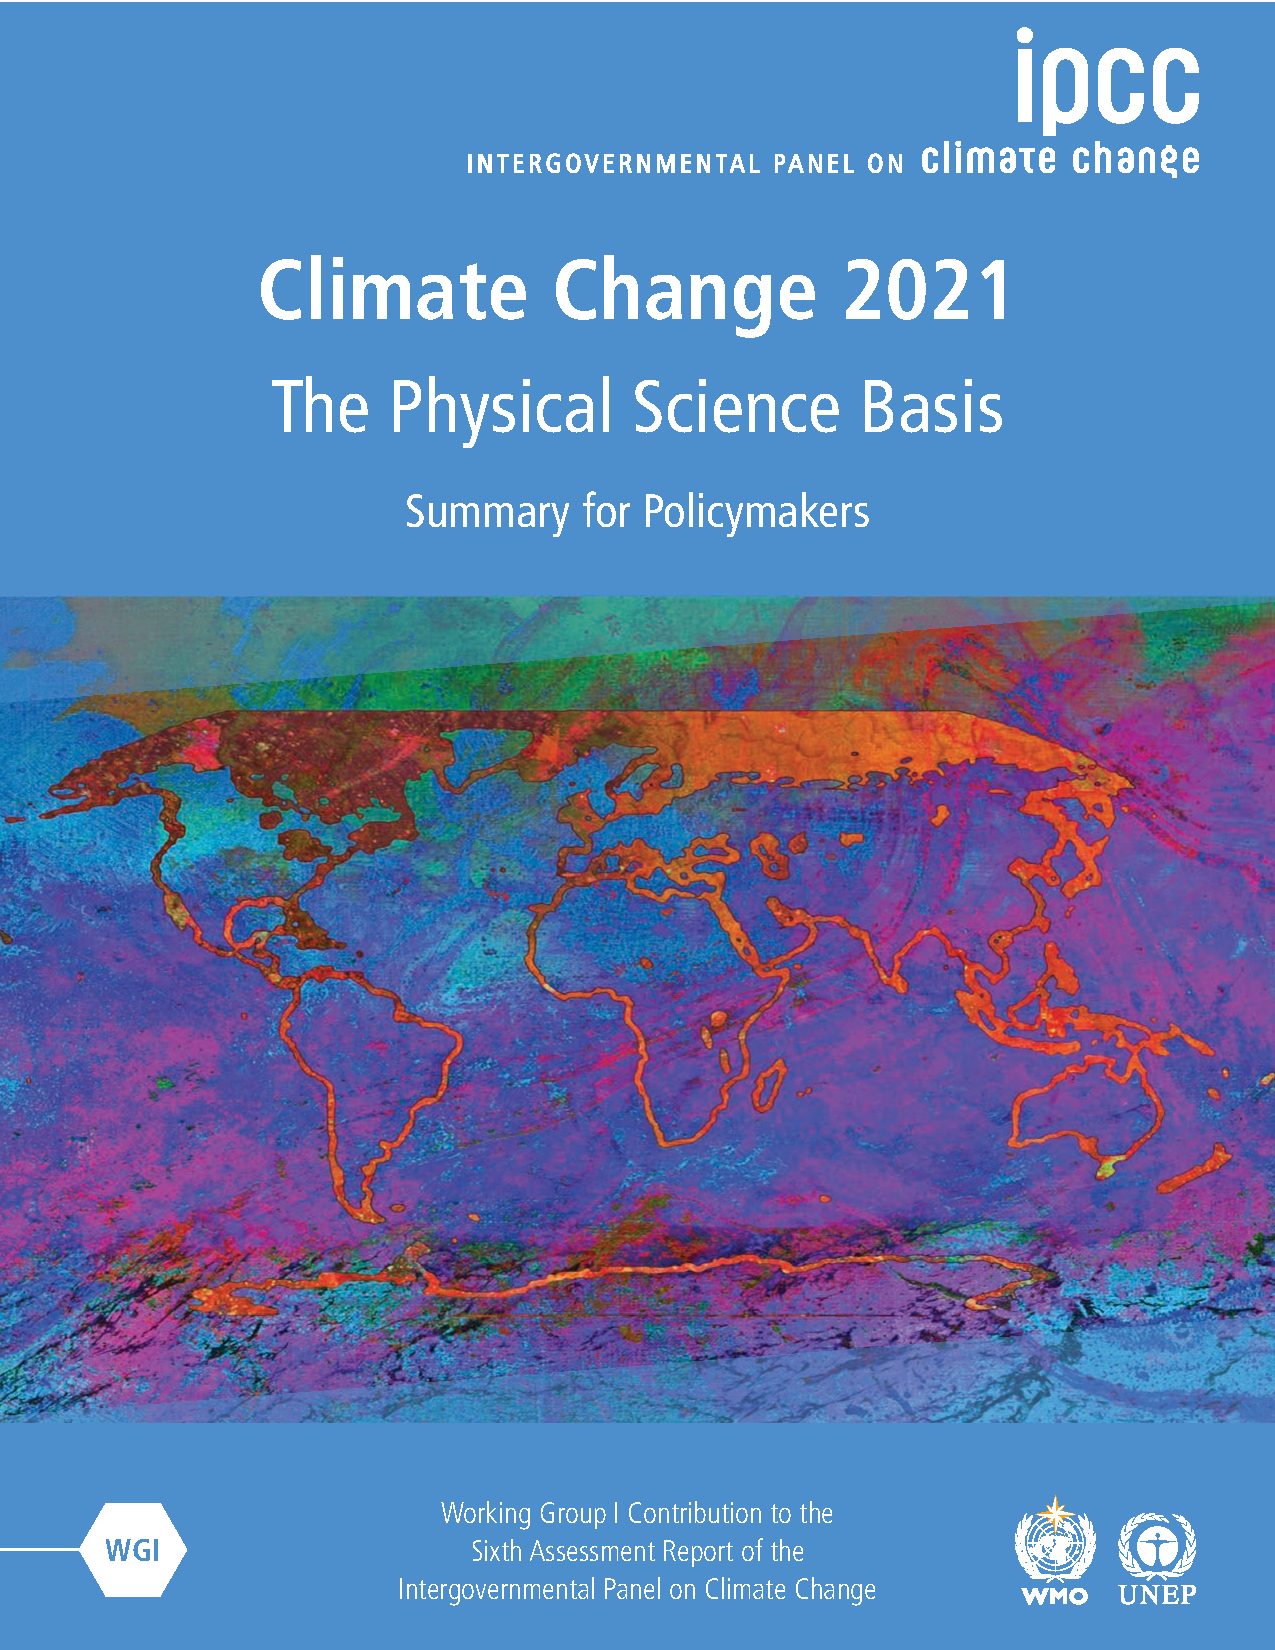
\includegraphics[height=5cm]{ar6-wg1}
      \end{figure}
    \end{column}
    \begin{column}{.6\linewidth}
      \begin{itemize}
      \item multi-model ensemble
      \item Ice Sheet Model Intercomparison Project for CMIP6 (ISMIP6), led by S. Nowicki, H. Goelzer, H. Seroussi, T. Payne and many more
      \item other efforts: ABUMIP, LARMIP-2, MISMIP+, etc.
      \end{itemize}
        \includegraphics<1>[width=2.5cm]{ismip6_logo}
    \end{column}
  \end{columns}
\end{frame}


\part{What's going on?}
\frame{\partpage}

\begin{frame}{A closer look: Greenland}
  \begin{figure}
    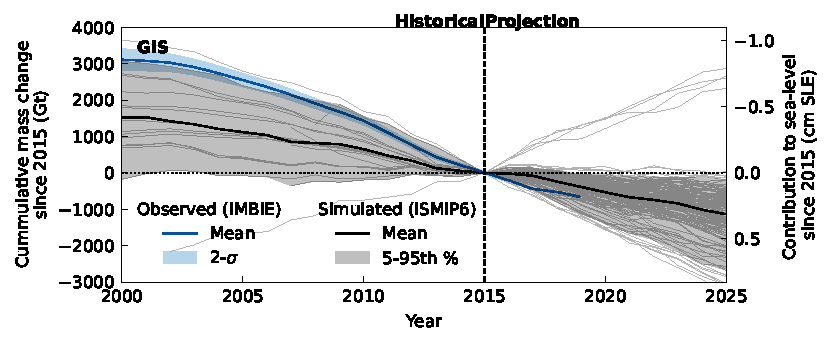
\includegraphics[width=\textwidth]{GIS_historical}
    \caption{Aschwanden, Brinkerhoff, Bartholomaus, \& Truffer (2021)}
  \end{figure}
  \begin{columns}[c]
    \begin{column}{.5\textwidth}
      \begin{minipage}[t][.5\textheight][t]{\textwidth}
        \alert{Almost all historical simulations under-estimate modern mass loss}
      \end{minipage}
    \end{column}
    \begin{column}{.25\textwidth}
    \end{column}
  \end{columns}
\end{frame}

\begin{frame}{A closer look: Antarctica}
  \begin{figure}
    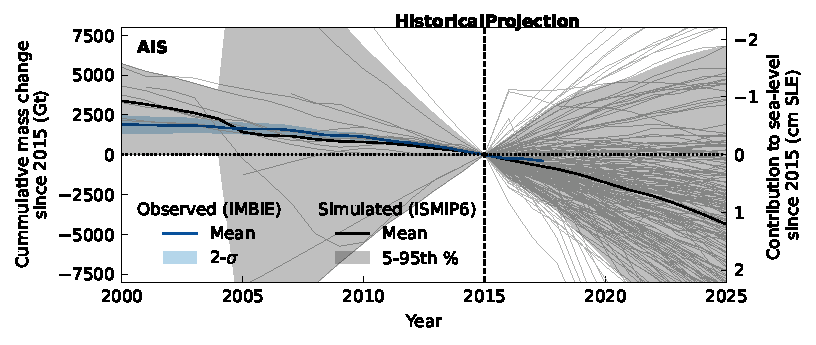
\includegraphics[width=\textwidth]{AIS_historical}
    \caption{Aschwanden, Brinkerhoff, Bartholomaus, \& Truffer (2021)}
  \end{figure}
  \begin{columns}[c]
    \begin{column}{.5\textwidth}
      \begin{minipage}[t][.5\textheight][t]{\textwidth}
        \alert{Spread in simulations much larger than observational uncertainty}
      \end{minipage}
    \end{column}
    \begin{column}{.25\textwidth}
    \end{column}
  \end{columns}
\end{frame}


\begin{frame}{Try it yourself}
  \begin{figure}
    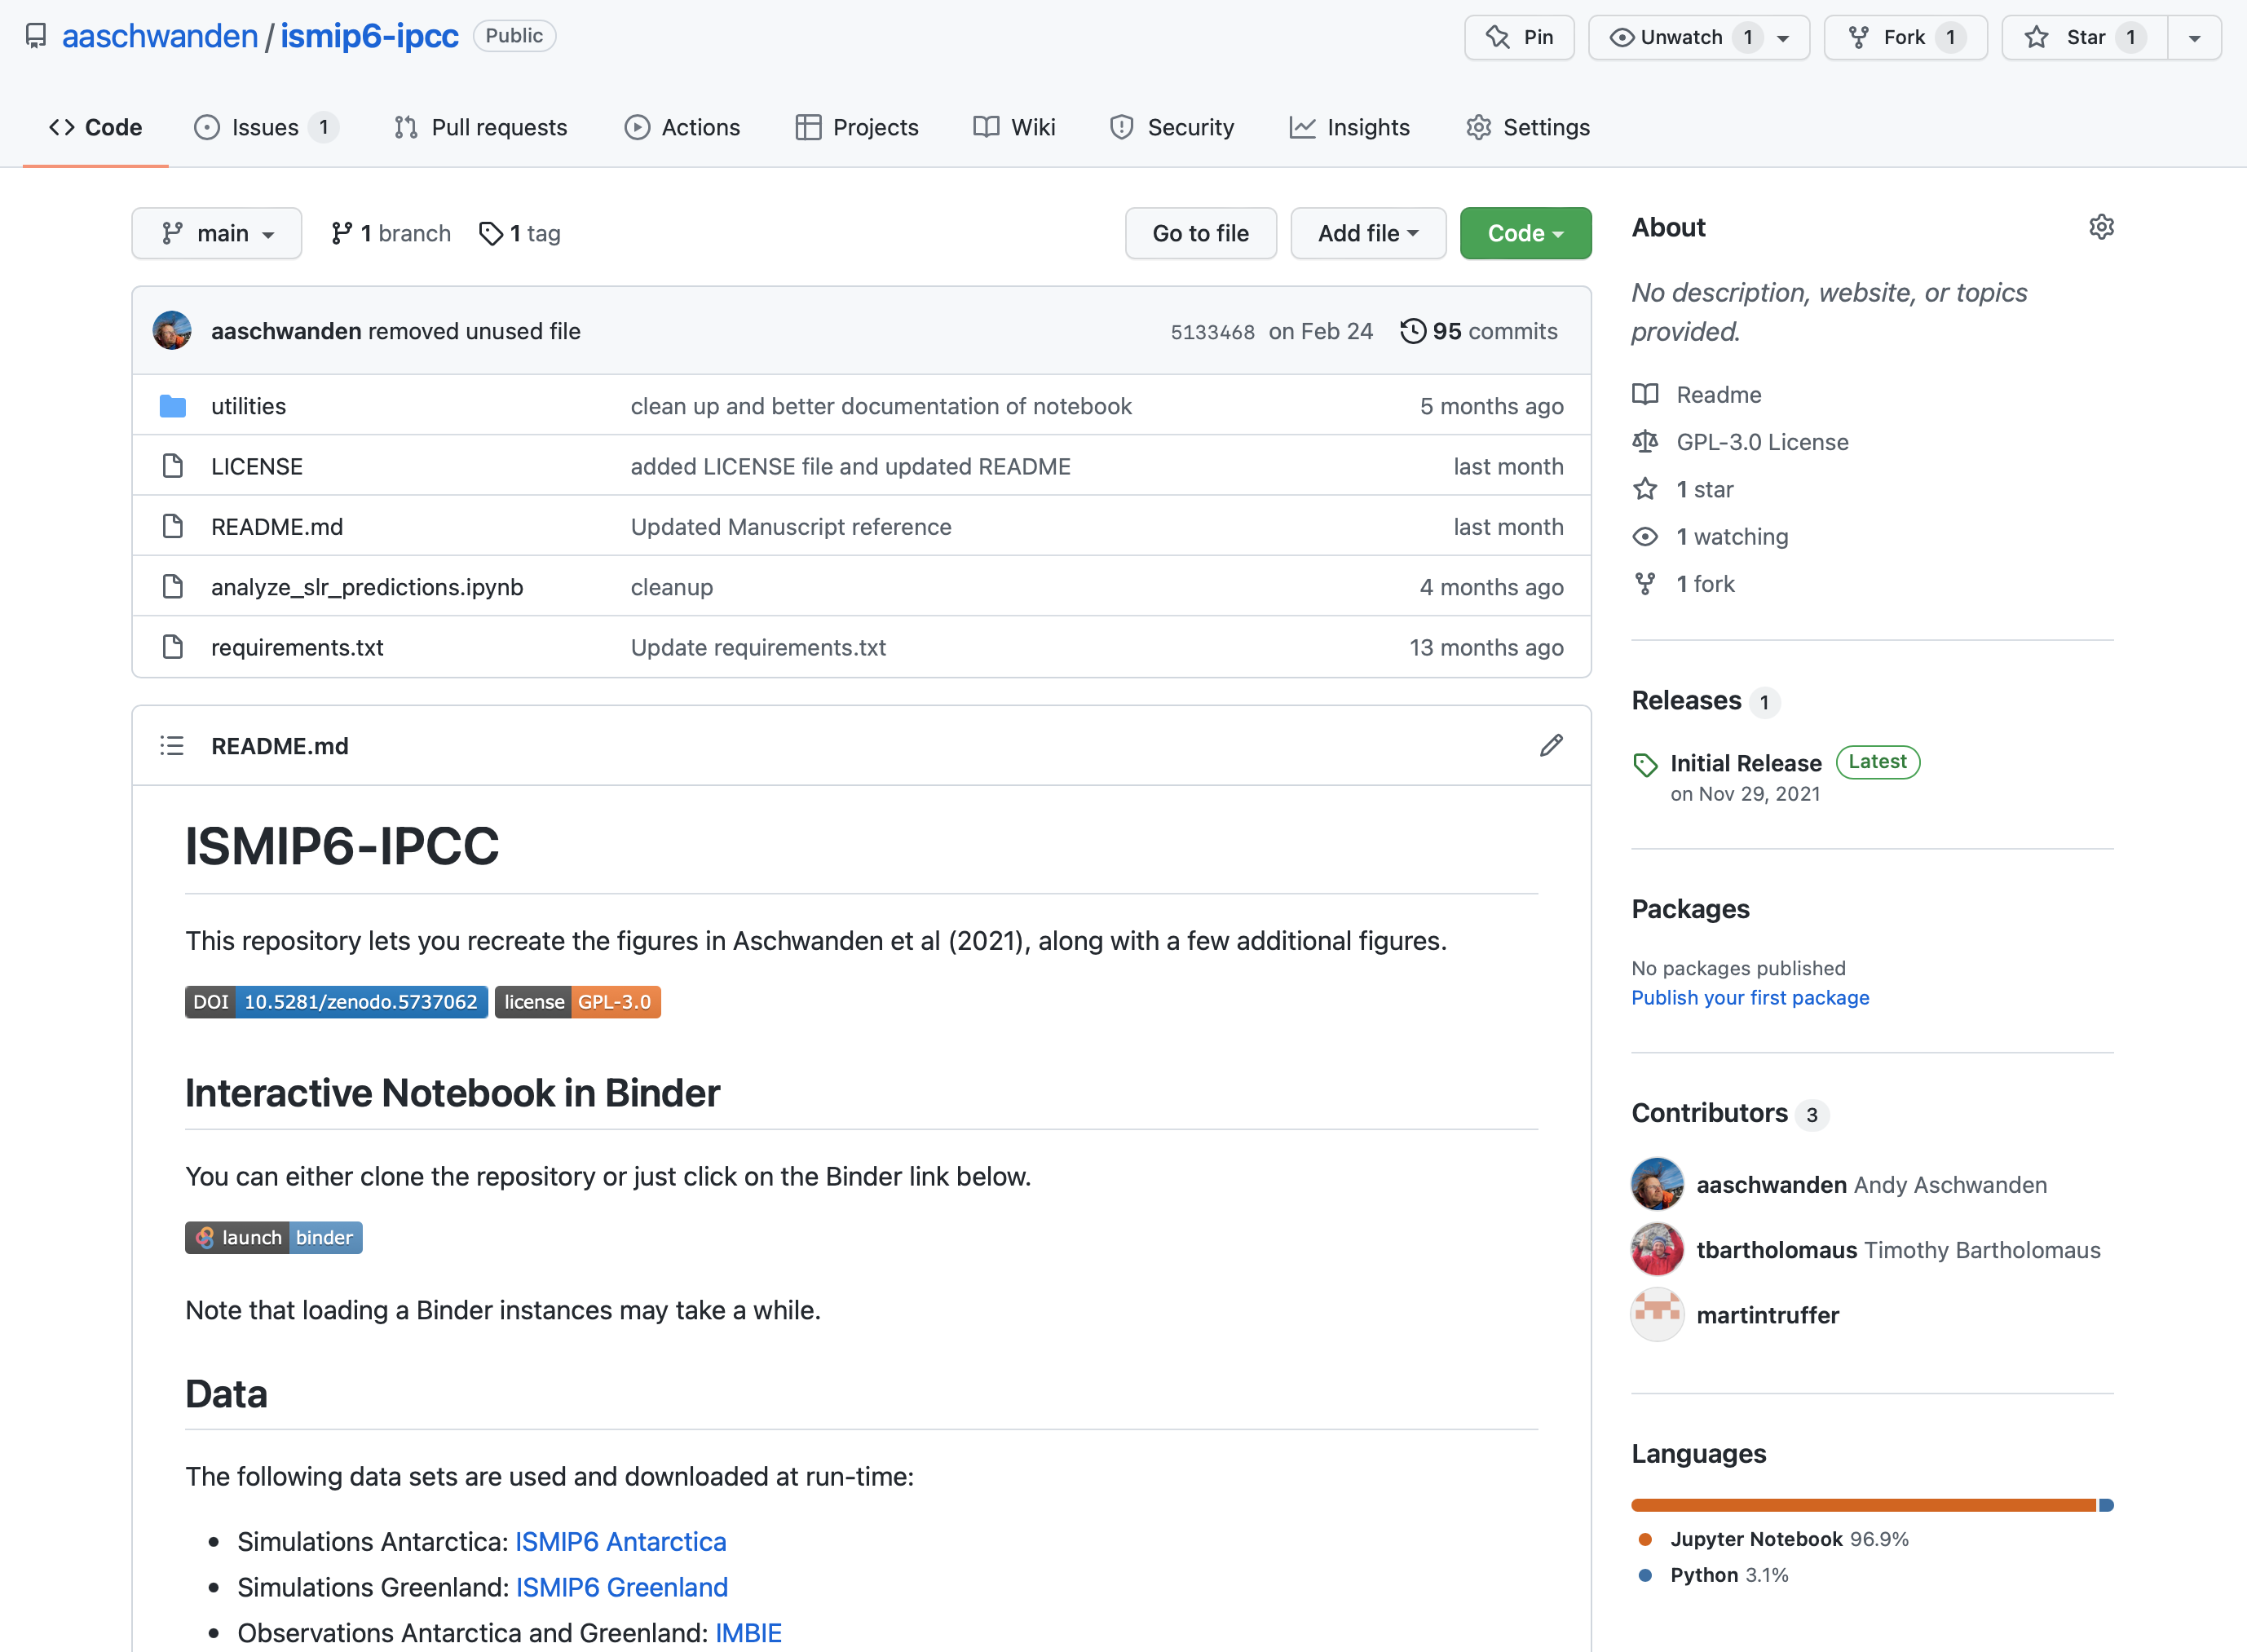
\includegraphics[width=.85\textwidth]{ismip6-ipcc-github-repo}
  \end{figure}
\end{frame}



\part{A path forward}

\frame{\partpage}

\setbeamertemplate{background canvas}
  {
}

\begin{frame}{2 key requirements}
Accurate predictions of the cryosphere's contribution to sea level require that models:
\begin{enumerate}
    \item Fully characterize uncertainties in model structure, parameters, initial conditions, and boundary conditions.
    \item Yield simulations that fit observations within observational uncertainty. 
\end{enumerate}
  \begin{figure}
    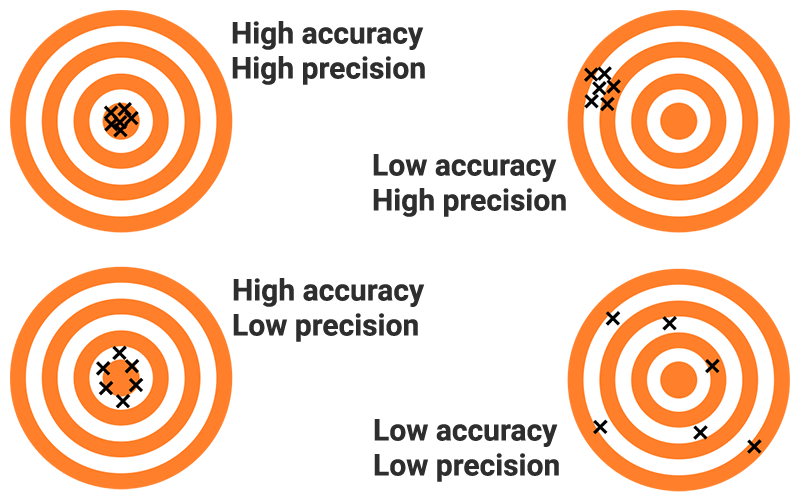
\includegraphics[width=0.4\textwidth]{difference-accuracy-and-precision}
  \end{figure}
  \begin{itemize}
    \item \alert{No new ideas used here.}
  \end{itemize}
\end{frame}

\begin{frame}{The first large ensemble projections for Greenland}
  \begin{figure}
    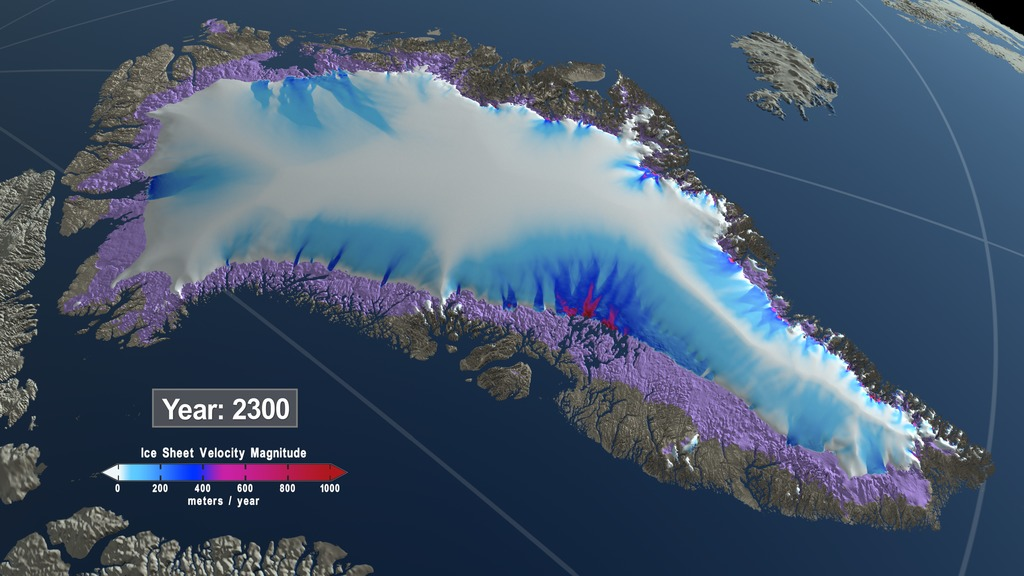
\includegraphics[width=0.8\textwidth]{Greenland_RCP_85_2008_2300_comp_4k.0293_print}
    \caption{NASA Scientific Visualization Studio. After Aschwanden et al. (2019).}
  \end{figure}
\end{frame}


\begin{frame}{AS19 Ensemble Projections}
  \begin{minipage}[t][4cm][t]{\textwidth}
    \begin{figure}
      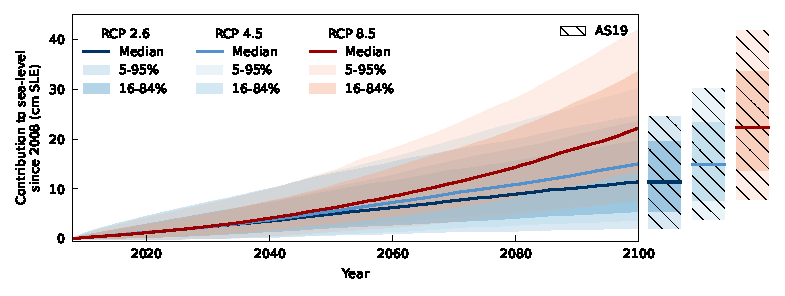
\includegraphics[height=4cm]{projection_as19_bars}
    \end{figure}
  \end{minipage}
  \alert{Prescribe pior distributions to assess parametric uncertainty}
  \begin{minipage}[t][3cm][t]{\textwidth}
    \begin{figure}
      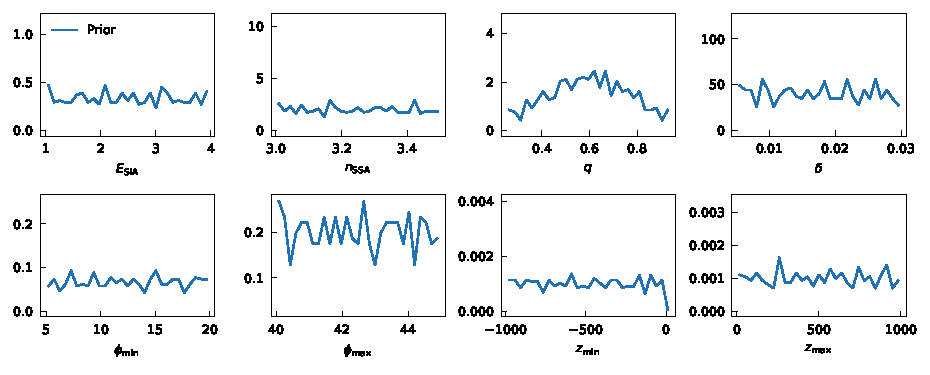
\includegraphics[height=3cm]{prior}
    \end{figure}
  \end{minipage}
\end{frame}



\begin{frame}{What's wrong with AS19}
  \begin{minipage}[t][4cm][t]{\textwidth}
    \begin{figure}
      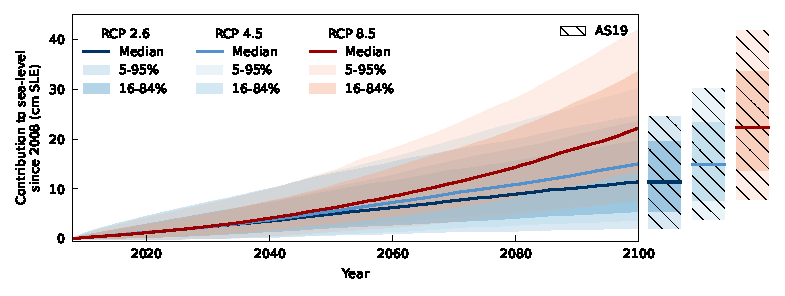
\includegraphics[height=4cm]{projection_as19_bars}
    \end{figure}
  \end{minipage}
  \centering{
  \alert{No conditioning on observations}}
  \begin{minipage}[t][3cm][t]{\textwidth}
  \end{minipage}
\end{frame}


\begin{frame}{Accounting for all sources of uncertainty}
    \begin{minipage}[t][2.75cm][t]{\textwidth}
    \begin{figure}
      \includegraphics<1->[height=2cm]{bayes_theorem}
    \end{figure}
  \end{minipage}
  We can cast this in a \alert{Bayesian} framework:
  \begin{figure}
    \includegraphics<1>[width=12cm]{slr-probability}    
  \end{figure}

\end{frame}


\begin{frame}{Sea-level contribution probability density function}
\begin{align}
P\left(\Delta_{2100} | \mathbf{D}, \mathcal{H}, \mathcal{F} \right) =&  \nonumber \\
 = &\int \underbrace{P\left(\Delta_{2100} | \mathbf{M},\mathcal{H}, \mathcal{F} \right)}_{\text{Projection}} \underbrace{P\left(\mathbf{M} | \mathbf{D},\mathcal{H}, \mathcal{F} \right)}_{\text{Calibration}}\, \mathrm{d} \mathbf{M},
    \label{eq:pos-pred}
\end{align}
$\mathbf{M}$: model parameters
\end{frame}

\begin{frame}{Probabilistic Calibration}
    \begin{minipage}[t][2.75cm][t]{\textwidth}
    \begin{figure}
      \includegraphics<1->[height=2cm]{bayes_theorem}
    \end{figure}
    \end{minipage}
    \begin{itemize}
    \item $P(\mathbf{M}|\mathbf{D},\mathcal{H})$ is analytically intractable
    \item we characterize the distribution with random samples (i.e. by approximating it with a histogram)
    \item We further subdivide this procedure into two sub-stages:
      \begin{enumerate}
      \item parameter calibration
      \item particle filtering (aka importance sampling, Bayesian calibration)
      \end{enumerate}
    \end{itemize}
\end{frame}





\begin{frame}{Probabilistic Calibration in two steps}
    \begin{minipage}[t][2cm][t]{\textwidth}
      \begin{block}{Which observations should we use?}
        \begin{itemize}
        \item<2-> use the quantity of interest: mass change
        \item<3> use quantity that contributes a lot to uncertainty: ice flow
        \end{itemize}
        \note[item]{}
      \end{block}
  \end{minipage}
    \begin{minipage}[t][6cm][t]{\textwidth}
        \begin{columns}[c]
    \begin{column}{.3\textwidth}
    \includegraphics<3>[height=5.5cm]{greenland-obs-rignot}
    \end{column}
    \begin{column}{.65\textwidth}
    \includegraphics<1->[height=3cm]{GIS_hist_only_obs}
    \end{column}
  \end{columns}

    \end{minipage}

\end{frame}


\begin{frame}{1. Ice Flow calibration}
  \begin{minipage}[t][6cm][t]{\textwidth}
    \begin{columns}[c]
      \begin{column}{.3\textwidth}
        \includegraphics[height=5.5cm]{greenland-obs-rignot}
      \end{column}
      \begin{column}{.65\textwidth}
        \begin{equation*}
          P(\mathbf{m}_{\mathrm{flow}}|\mathbf{u}_{\mathrm{obs}})
        \end{equation*}
        \begin{itemize}
        \item $\mathbf{m}_{\mathrm{flow}}$: parameters controlling ice flow
        \item $\mathbf{u}_{\mathrm{obs}}$: surface speed observations
        \end{itemize}
      \end{column}
    \end{columns}  
  \end{minipage}
\end{frame}


\begin{frame}{1. Ice Flow calibration: strategy}
\begin{itemize}
\item use Markov Chain Monte Carlo sampling (MCMC) to find the joint distribution of these parameters given observations.
\item think of the ice sheet model as a map $\mathcal{F}$ from a parameter vector $\mathbf{x}$ to surface speeds $\mathbf{Y}$
\begin{equation*}
\mathbf{Y} = \mathcal{F}(\mathbf{x})
\end{equation*}
\item running the forward model (PISM) is too expensive for MCMC
\item Generate a ``cheap'' surrogate model $\mathcal{G}$ such that
\begin{equation*}
\mathcal{G}(\mathbf{x}) \approx \mathcal{F}(\mathbf{x})
\end{equation*}
\item use the 4 layer Neural Network surrogate model by Brinkerhoff et al (2021), implemented in PyTorch
\end{itemize}
  \begin{figure}
    
\includegraphics[width=.35\textwidth]{neural-network}
  \end{figure}
\end{frame}



\begin{frame}{1. Ice Flow calibration: dimensionality reduction}
  \alert{Challenge $\mathbf{Y}$ is not a scalar}:
\begin{eqnarray*}
\mathbf{x} = \{x_1, x_2,\ldots,x_n\}, & n = 8, \\ 
\mathbf{Y} = \{Y_1, Y_2, \ldots,Y_m \},& m \ge 10^6
\end{eqnarray*}
\vspace{-1.5em}
\begin{block}{SVD / PCA / EOF}
\begin{itemize}
\item decompose training data into ``eigen-glaciers'' using Principal Component Analysis (``eigen faces'' in picture analysis)
\item we only need to simulate the first $\sim$100 eigen-coefficients to capture 99.95\% of the variance
\item we have reduced the problem from 10$^6$ to $\sim$100 unknowns.
\end{itemize}
\vspace{-0.5em}
\end{block}
\begin{figure}
  \includegraphics<1->[height=6cm]{eigenglaciers_0}
\end{figure}
\end{frame}


\begin{frame}{1. Ice Flow calibration: training data}
  \begin{columns}[c]
    \begin{column}{0.5\textwidth}
      \begin{figure}
        \includegraphics<1->[width=.95\textwidth]{calib-speeds}
      \end{figure}
    \end{column}
    \begin{column}{.5\textwidth}
      \begin{itemize}
      \item select 8 relevant parameters
      \item define a prior probability distribution for each parameter
      \item draw 1,000 samples using Sobol Sequences
      \item run PISM 1,000 times
      \end{itemize}
    \end{column}
  \end{columns}  
\end{frame}




\begin{frame}{1. Ice Flow: surrogate model and sampling}
  \begin{figure}
    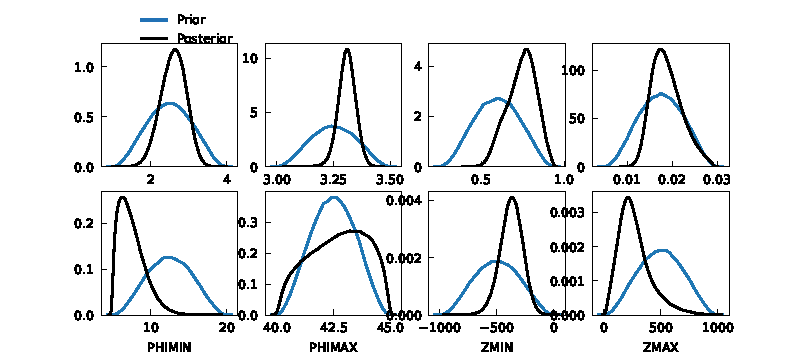
\includegraphics[width=0.75\textwidth]{prior_posterior}
  \end{figure}
  \begin{itemize}
  \item using the surrogate model, create 1,000,000 member strong ensemble
  \item run MCMC sampling given observations
  \item what you get are posterior distributions of the parameters
  \item these distributions best fit the surface speeds observations
  \end{itemize}
\end{frame}

\begin{frame}{Use posterior as new prior}
\begin{columns}[c]
    \begin{column}{.5\textwidth}
      \begin{figure}
        \includegraphics<1>[height=7.5cm]{sle_pdf_w_obs_as19_2020.pdf}
        \includegraphics<2>[height=7.5cm]{sle_pdf_w_obs_as19flow_2020.pdf}
    \end{figure}
    \end{column}
    \begin{column}{.5\textwidth}
      \begin{figure}
    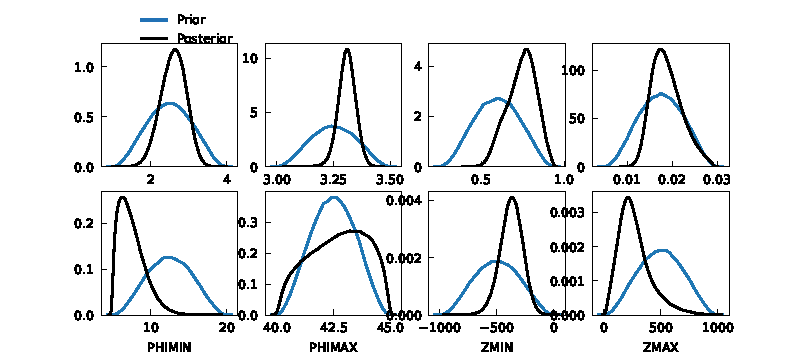
\includegraphics[width=0.85\textwidth]{prior_posterior}
  \end{figure}

  \begin{itemize}
  \item<1> create 500 samples from posterior
  \item<1> rerun PISM 500x, wait
  \item<2> get new projections conditioned on surface speeds
  \item<2> find reduced variance
  \end{itemize}
    \end{column}
  \end{columns}

\end{frame}


\begin{frame}{2. Mass Loss: Particle Filtering}
  \begin{minipage}[t][4cm][t]{\textwidth}
    \begin{figure}
    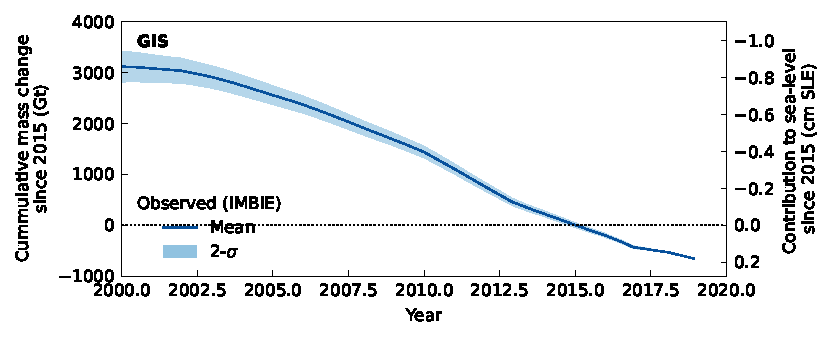
\includegraphics[height=4cm]{GIS_hist_only_obs}
    \end{figure}
  \end{minipage}
  \begin{itemize}
  \item  weight members based on their likelihood relative to observations of mass change.
  \item resample simulations proportionally to these likelihoods to create a new ensemble that is consistent with respect to both  observations of surface speed and mass change to within observational uncertainty
  \end{itemize}
\end{frame}


\begin{frame}{Posterior distributions}
\begin{columns}[c]
    \begin{column}{.5\textwidth}
    \begin{figure}
      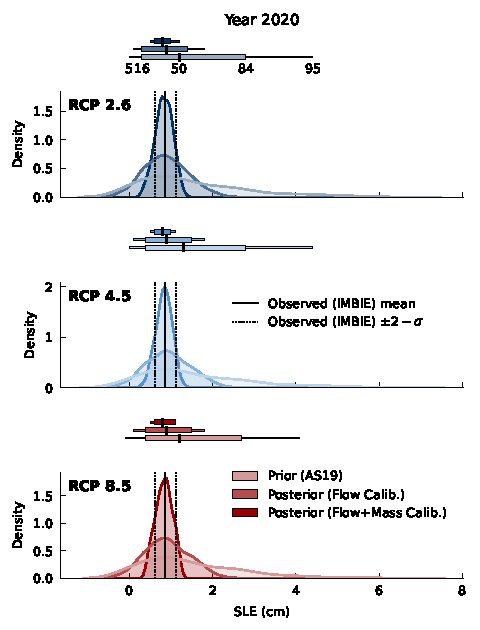
\includegraphics[height=7.75cm]{sle_pdf_w_obs_calibrated_2020.pdf}
    \end{figure}
    \end{column}
    \begin{column}{.5\textwidth}
  \begin{itemize}
  \item fully calibrated posterior agrees well with observations (IMBIE)
    \end{itemize}
    \end{column}
  \end{columns}
 \end{frame}


\begin{frame}{Calibrated 2100 Projections}
    \begin{figure}
      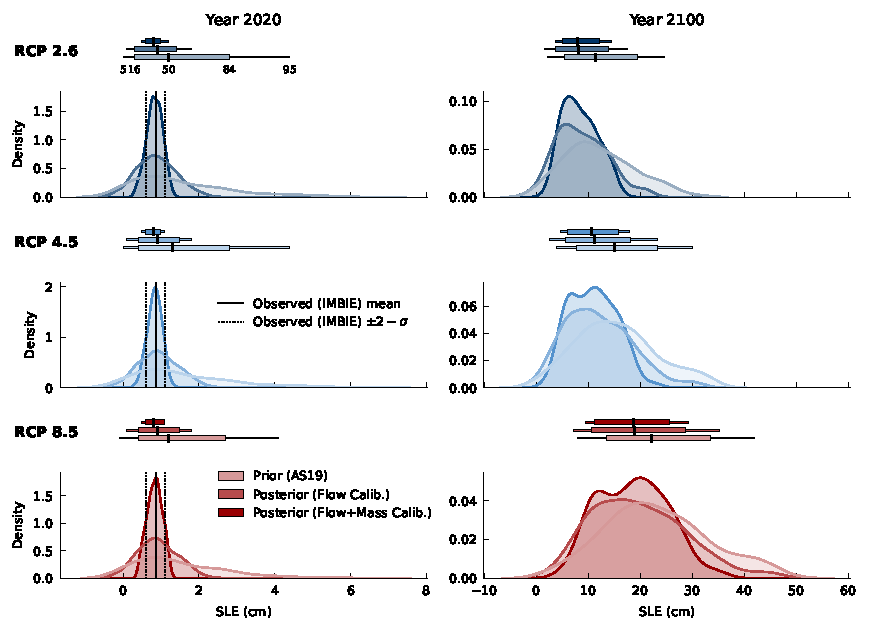
\includegraphics[height=7.75cm]{sle_pdf_w_obs_2020_2100}
    \end{figure}
\end{frame}


\begin{frame}{Initial idea 2020: Kalman Smoother}
  \begin{figure}
    \includegraphics<1->[width=\textwidth]{flowchart-kalman-smoother}
  \end{figure}
\end{frame}

\begin{frame}{Current idea 2022: Particle Filter}
  \begin{figure}
    \includegraphics<1>[width=\textwidth]{flowchart-particle-filter}
    \includegraphics<2>[width=\textwidth]{flowchart-particle-filter-tasks}
  \end{figure}
\end{frame}


  
\setbeamertemplate{background canvas}
  {
     \tikz{\node[inner sep=0pt,opacity=1.0] {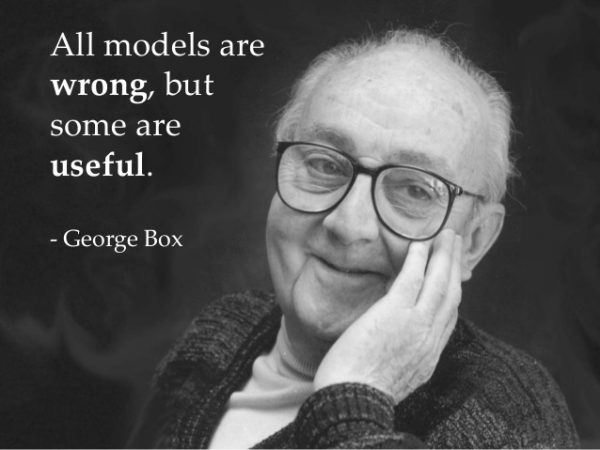
\includegraphics[height=\paperheight]{all-models-are-wrong}};}
}

\begin{frame}{}
\end{frame}


\end{document}
